%% bei Standalone in documentclass noch:
% \RequirePackage{luatex85}

\documentclass[captions=tableheading, titlepage= firstiscover, parskip = half , bibliography=totoc]{scrartcl}
%paper = a5 für andere optinen
% titlepage= firstiscover
% bibliography=totoc für bibdateien
% parskip=half  Veränderung um Absätze zu verbessern

\usepackage{scrhack} % nach \documentclass
\usepackage[aux]{rerunfilecheck}
\usepackage{polyglossia}
\usepackage[style=numeric, backend=biber]{biblatex} % mit [style = alphabetic oder numeric] nach polyglossia
\addbibresource{lit.bib}
\setmainlanguage{german}

\usepackage[autostyle]{csquotes}
\usepackage{amsmath} % unverzichtbare Mathe-Befehle
\usepackage{amssymb} % viele Mathe-Symbole
\usepackage{mathtools} % Erweiterungen für amsmath
\usepackage{fontspec} % nach amssymb
% muss ins document: \usefonttheme{professionalfonts} % für Beamer Präsentationen
\usepackage{longtable}

\usepackage[
math-style=ISO,    % \
bold-style=ISO,    % |
sans-style=italic, % | ISO-Standard folgen
nabla=upright,     % |
partial=upright,   % /
]{unicode-math} % "Does exactly what it says on the tin."
\setmathfont{Latin Modern Math}
% \setmathfont{Tex Gyre Pagella Math} % alternativ

\usepackage[
% die folgenden 3 nur einschalten bei documenten
locale=DE,
separate-uncertainty=true, % Immer Fehler mit ±
per-mode=symbol-or-fraction, % m/s im Text, sonst \frac
]{siunitx}

% alternativ:
% per-mode=reciprocal, % m s^{-1}
% output-decimal-marker=., % . statt , für Dezimalzahlen

\usepackage[
version=4,
math-greek=default,
text-greek=default,
]{mhchem}

\usepackage[section, below]{placeins}
\usepackage{caption} % Captions schöner machen
\usepackage{graphicx}
\usepackage{grffile}
\usepackage{subcaption}

% \usepackage{showframe} Wenn man die Ramen sehen will

\usepackage{float}
\floatplacement{figure}{htbp}
\floatplacement{table}{htbp}

\usepackage{mhchem} %chemische Symbole Beispiel: \ce{^{227}_{90}Th+}


\usepackage{booktabs}

 \usepackage{microtype}
 \usepackage{xfrac}

 \usepackage{expl3}
 \usepackage{xparse}

 % \ExplSyntaxOn
 % \NewDocumentComman \I {}  %Befehl\I definieren, keine Argumente
 % {
 %    \symup{i}              %Ergebnis von \I
 % }
 % \ExplSyntaxOff

 \usepackage{pdflscape}
 \usepackage{mleftright}

 % Mit dem mathtools-Befehl \DeclarePairedDelimiter können Befehle erzeugen werden,
 % die Symbole um Ausdrücke setzen.
 % \DeclarePairedDelimiter{\abs}{\lvert}{\rvert}
 % \DeclarePairedDelimiter{\norm}{\lVert}{\rVert}
 % in Mathe:
 %\abs{x} \abs*{\frac{1}{x}}
 %\norm{\symbf{y}}

 % Für Physik IV und Quantenmechanik
 \DeclarePairedDelimiter{\bra}{\langle}{\rvert}
 \DeclarePairedDelimiter{\ket}{\lvert}{\rangle}
 % <name> <#arguments> <left> <right> <body>
 \DeclarePairedDelimiterX{\braket}[2]{\langle}{\rangle}{
 #1 \delimsize| #2
 }

\setlength{\delimitershortfall}{-1sp}

 \usepackage{tikz}
 \usepackage{tikz-feynman}

 \usepackage{csvsimple}
 % Tabellen mit \csvautobooktabular{"file"}
 % muss in table umgebung gesetzt werden


% \multicolumn{#Spalten}{Ausrichtung}{Inhalt}

\usepackage{hyperref}
\usepackage{bookmark}
\usepackage[shortcuts]{extdash} %nach hyperref, bookmark

\newcommand{\ua}[1]{_\symup{#1}}
\newcommand{\su}[1]{\symup{#1}}


%\begin{document}

\section{Auswertung}

Im Folgendem werden die Messergebnisse ausgewertet und in geeigneter
Weise visualisert.

\subsection{Grenzfrequenzen}

Die verwendete Apparatur hatte die folgenden Werte.

\begin{align}
  \label{L}
  L &= \SI{1,217}{\milli\henry}\\
  \label{C1}
  C_1 &= \SI{20,13}{\nano\farad}\\
  \label{C2}
  C_2 &= \SI{9,41}{\nano\farad}
\end{align}

Diese Daten wurden ohne Fehler angegeben und werden deshalb als fehlerfrei
angenommen. In der $LC$-Kettenschaltung wurde der Kondensator mit der
Kapazität $C_1$ verwendet.

Es gelten die folgenden Zusammenhänge für die Apparaturkonstanten und die
Grenzrequenzen.

\begin{align}
  \label{eqn:omega_C_grenz}
  \omega_{Grenz,C} &= \frac{2}{\sqrt{L\cdot C_1}} \\
  \label{eqn:omega_C_2_grenz}
  \omega_{Grenz,C_1C_2}^{akustisch} &= \sqrt{\frac{2}{L\cdot C_2}} \\
  \label{eqn:omega_C_1_grenz}
  \omega_{Grenz,C_1C_2}^{optisch} &= \sqrt{\frac{2}{L\cdot C_1}} \\
\end{align}

Mittels \eqref{eqn:omega_C_grenz}, \eqref{eqn:omega_C_2_grenz} und
\eqref{eqn:omega_C_1_grenz} ergeben sich die Werte:

\begin{align*}
  \omega_{Grenz,C} &= \num{404075}\si{\hertz}\\
  \omega_{Grenz,C_1C_2}^{akustisch} &= \num{285724}\si{\hertz}\\
  \omega_{Grenz,C_1C_2}^{optisch} &= \num{417902}\si{\hertz}.\\
\end{align*}

Mit Hilfe des $XY$-Scheibers wurden die Grenzfrequenzen der $LC$-Kettenschaltung
und der $LC_1C_2$-Kettenschaltung visualisiert. Die Diagramme sind
logarithmisch. Durch Ermitteln der Frequenzen an bestimmten Stellen der
Grafik kann eine exponentielle Regressionsrechnung gemacht werden.
Damit ist einen Zusammenhang zwischen den Messdaten und vom Generator durchlaufenden
Frequenzen bekannt.

Die Ausgleichsrechnung wurde mithilfe des \emph{Python}-Paketes
\emph{curve\_Fit} bewerkstelligt. Die Funktion hatte die Gestalt:

\begin{equation}
  \nu(t) = a\cdot e^{bx}+c.
\end{equation}

\begin{figure}
  \includegraphics[width=\textwidth]{Ceinzeln.pdf}
  \caption{Durchlasskurve einer Kettenschaltung mit einem Typ Kondensator}
  \label{fig:Ceinzeln}
\end{figure}

\begin{figure}
  \includegraphics[width=\textwidth]{C1C2.pdf}
  \caption{Durchlasskurve einer Kettenschaltung mit zwei verschiedenen Typen Kondensator}
  \label{fig:C1C2}
\end{figure}


Die Messungen der Durchlasskurve ergaben die folgenden Werte.

\FloatBarrier
\floatplacement{table}{htbp}
\begin{table}
 \centering
 \begin{tabular}[width=\textwidth]{S| S[table-format=4.0] S[table-format=5.0] S[table-format=5.0] S[table-format=5.0] S[table-format=5.0] S[table-format=5.0] S[table-format=5.0]}
    \midrule
    $\nu_C$ \text{\;in\;} $\si{\hertz}$ & 1338 & 2055 & 2843 & 3730 & 5023 & 6471 & 8624 \\
    $\nu_{C_1C_2}$ \text{\;in\;} $\si{\hertz}$ & 7345 & 10478 & 21072 & 30336 & 50353 & 79169 \\
    \bottomrule
\end{tabular}
  \caption{Messdaten der Durchlasskurve}
  \label{tab:Durchlasskurve}
\end{table}
\FloatBarrier

Es ergeben sich mittels der Messdaten der Tabelle \ref{tab:Durchlasskurve}
die folgenden Funktionen.

\begin{align}
  \label{eqn:Ausgleichsrechnung_exp_1}
  \nu_{C}(x) &= ((13984\pm 1701)\si{\hertz})\cdot e^{(0,08\pm 0,005)\frac{1}{\si{\centi\meter}}\cdot x} - (5155\pm 2006)\si{\hertz} \\
  \label{eqn:Ausgleichsrechnung_exp_2}
  \nu_{C_1C_2}(x) &= ((64117\pm 5474)\si{\hertz})\cdot e^{(0,15\pm 0,005)\frac{1}{\si{\centi\meter}}\cdot x}-(20547\pm 7703)\si{\hertz}
\end{align}

Anhand der Graphen kann die Grenzfrequenz abgelesen werden, indem der
Abstand vermessen wird. Die Messung wurde mit einem Lineal gemacht
und ergibt für die $LC$-Kettenschaltung einen Wert von ca.
$\SI{17,2}{\centi\meter}$. Die Messung der Grenzfrequenzen der
$LC_1C_2$-Kettenschaltung ergab für den akustischen Zweig eine
Grenzfrequenz bei $\SI{11}{\centi\meter}$ und für den optischen Zweig eine
Grenzfrequenz bei  $\SI{12,2}{\centi\meter}$.

Für die Grenzfrequenzen ergeben sich damit die Werte:

\begin{align}
  \omega_{Grenz,C} &= \num{50224,00}\si{\hertz}\\
  \omega_{Grenz,C_1C_2}^{akustisch} &= \num{311361,75}\si{\hertz}\\
  \omega_{Grenz,C_1C_2}^{optisch} &= \num{376566,51}\si{\hertz}
\end{align}

\subsection{Dispersionskurven}

Mit den Angaben \eqref{L}, \eqref{C1} und \eqref{C2} kann die Dispersionskurve
der $LC-Kette$ und der $LC_1C_2$-Kette über die Funktionen \eqref{eqn:RelationC}
und \eqref{eqn:RelationC1C2} bestimmt werden.
Die Messdaten wurden in das Diagramm mit eingetragen. Bei allen Werten die eine
Phasenverschiebung von über $\frac{\pi}{2}$ haben wurde die Phasenverschiebung
mit $\frac{\pi}{2}$ subtrahiert und an der $y$-Achse gespiegelt,
da die Dispersionskurve $\frac{\pi}{2}$-Periodisch ist.

\begin{figure}
  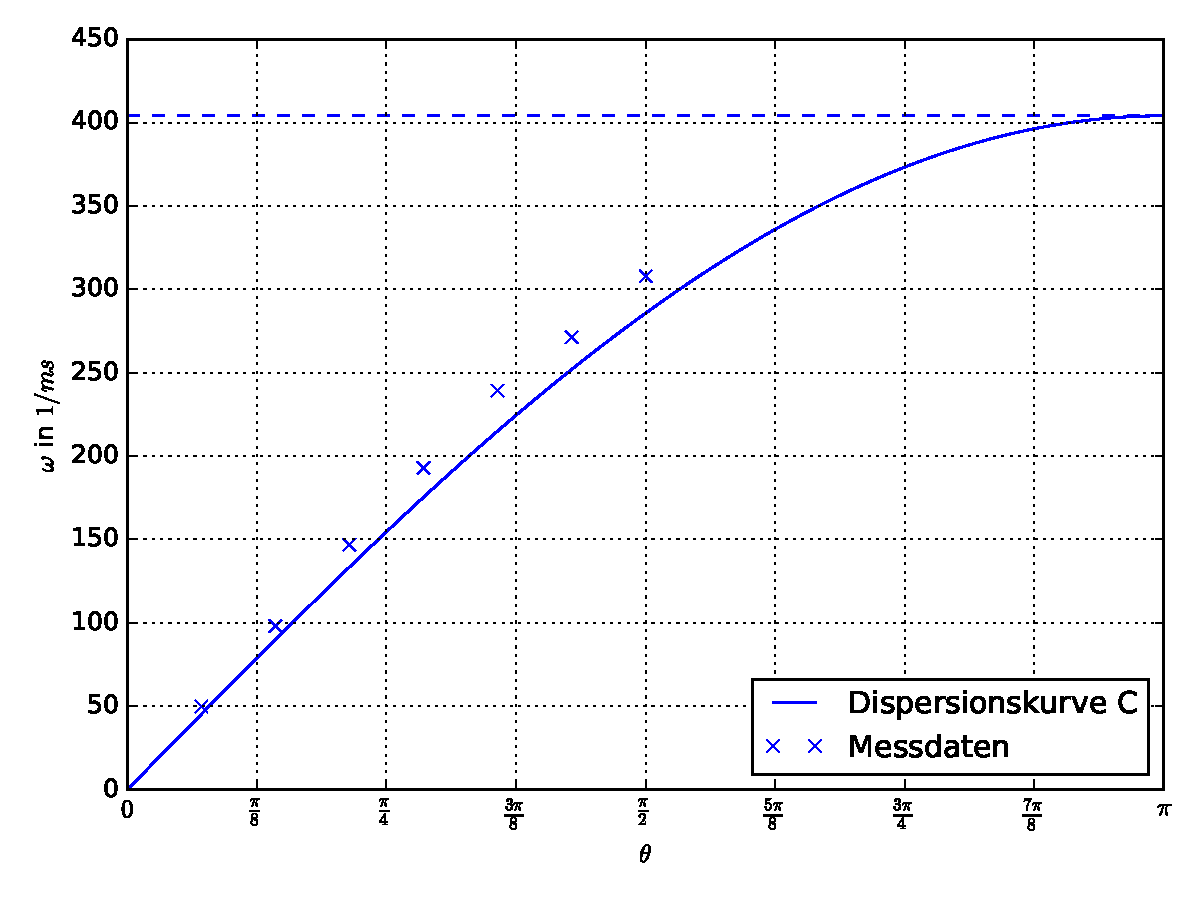
\includegraphics[width=\textwidth]{Dispersionskurve_C.pdf}
  \caption{Dispersionskurve der $LC$-Kettenschaltung}
  \label{fig:DispersionC}
\end{figure}

In Abb. \ref{fig:DispersionC} ist die Kreisfrequenz $\omega$ der Phasenverschiebung
pro Glied $\theta$ gegenüber aufgetragen. Die in dem Diagramm eingetragenen
Messdaten sind in Tabelle \ref{tab:Dispersionsrelation} in der Spalte
der $LC$-Kette dargestellt. An der Theoriekurve ist zu erkennen, dass die Kreizfrequenz
mit steigender Phasenverschiebung pro Glied sich der Grenzfrequenz asymptotisch
nähert. Grenzfrequenz ergibt sich aus dem folgendem Zusammenhang:

\begin{equation}
  \label{eqn:Grenzfrequenz}
  \omega_{Grenz} = \frac{2}{\sqrt{L\cdot C_1}}
\end{equation}

Die Messdaten liegen in guter Näherung auf der Theoriekurve.
Nur Werte bis zu einer Phasenverschiebung pro Glied von $\frac{\pi}{2}$
konnten gemessen werden. Alle Werte darüberhinaus waren nicht mehr messbar.

\FloatBarrier
\begin{figure}
  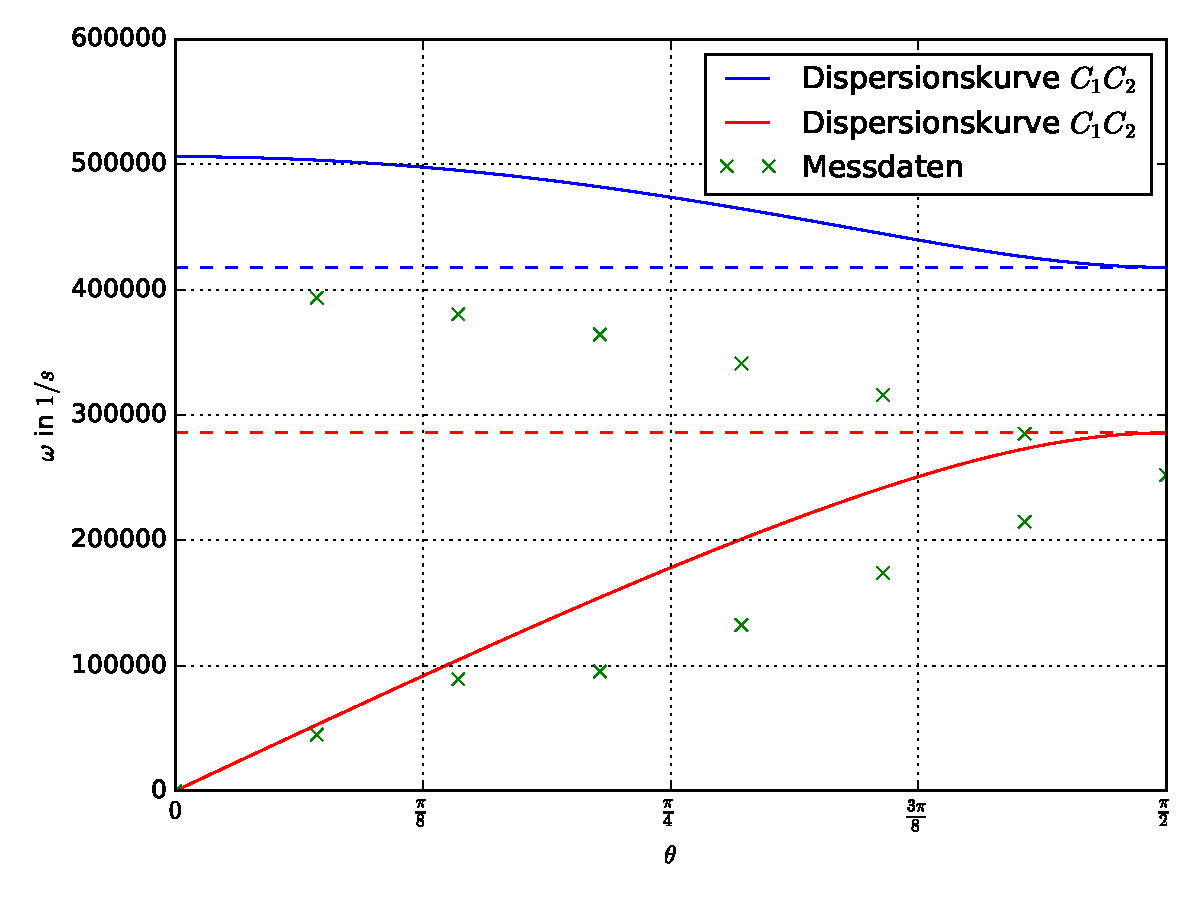
\includegraphics[width=\textwidth]{Dispersionskurve_C1C2.pdf}
  \caption{Dispersionskurve der $LC_1C_2$-Kettenschaltung}
  \label{fig:DispersionC1C2}
\end{figure}
\FloatBarrier

Das Diagramm \ref{fig:DispersionC1C2} zeigt die Dispersionskurve der $LC_1C_2$-Kette.
Tabelle \ref{tab:Dispersionsrelation} enthält in der Spalte zur $LC_1C_2$-Kette
die eingetragenen Messdaten. Der Theoriegraph besteht zum einen aus dem
optischen Ast und zum anderen aus dem akkusitschen Ast. Die Messdaten weichen deutlich
von den Theoriewerten ab. Auf diese Abweichung wird speziell nocheinmal in der
Diskussion eingegangen.

Die Messdaten der Dispersionsrelation sind in Tabelle \ref{tab:Dispersionsrelation}
dargestellt.

\floatplacement{table}{htbp}
\begin{table}
 \centering
 \sisetup{table-format=5.0}
 \begin{tabular}[width=\textwidth]{S S S}
     \toprule
      {Verschiebung} & {$\nu_C$} & {$\nu_{C_1C_2}$}\\
     \midrule
      0 & 0 & 0 \\
      1\pi & 7927 & 7158 \\
      2\pi & 15610 & 14188 \\
      3\pi & 23372 & 21078 \\
      4\pi & 30703 & 27714 \\
      5\pi & 38072 & 34188 \\
      6\pi & 43171 & 40094 \\
      7\pi & 49000 & 45378 \\
      8\pi & \text{--} & 50298 \\
      9\pi & \text{--} & 54295 \\
      10\pi & \text{--} & 57976 \\
      11\pi & \text{--} & 60550 \\
      12\pi & \text{--} & 62625 \\
      \bottomrule
\end{tabular}
  \caption{Messdaten der Dispersionsrelation}
  \label{tab:Dispersionsrelation}
\end{table}

\subsection{Phasengeschwindigkeit}

Anhand der Dispersionsrelation und der gemessenen Eigenfrequeunzen aus Tabelle
\ref{tab:Dispersionsrelation} lässt sich die Phasengeschwindigkeit über die
Formel \eqref{eqn:Phasengeschwindigkeit} berechnen.
Die Theoriekurve und die Werte, die sich aus den Messungen ergeben sind in
dem Diagramm \ref{fig:Phasengesch} dargestellt.
Die Phasenverschiebung pro Glied $\theta$ berechnet sich durch:

\begin{equation}
  \label{eqn:theta}
  \theta = \frac{\pi n_i}{n}, i = 0,...,14
\end{equation}

Dabei ist $n$ die Anzahl der Kettenglieder.

\FloatBarrier
%\tiny{
\floatplacement{table}{htbp}
\begin{table}
 \centering
 \sisetup{table-format=6.0}
 \begin{tabular}[width=\textwidth]{S| S S S S S S S S}
    \midrule
    $\theta$ & 0 & $\frac{\pi}{14}$ & $\frac{\pi}{7}$ & $\frac{3\pi}{14}$ & $\frac{2\pi}{7}$ & $\frac{5\pi}{14}$ & $\frac{3\pi}{7}$ & $\frac{\pi}{2}$ \\
    $v_{Ph}$\text{\,in\,}$\frac{1}{rad}$ & \text{\,\,\,\,\,\,\,\,\,\,\,\,\,\,\,\,--} & 201524 & 200019 & 19412 & 193799 & 188791 & 184288 & 177700 \\
    \bottomrule
\end{tabular}
  \caption{Messdaten der Phasengeschwindigkeit}
  \label{tab:Phasengesch}
\end{table}
%}
\FloatBarrier

\begin{figure}
  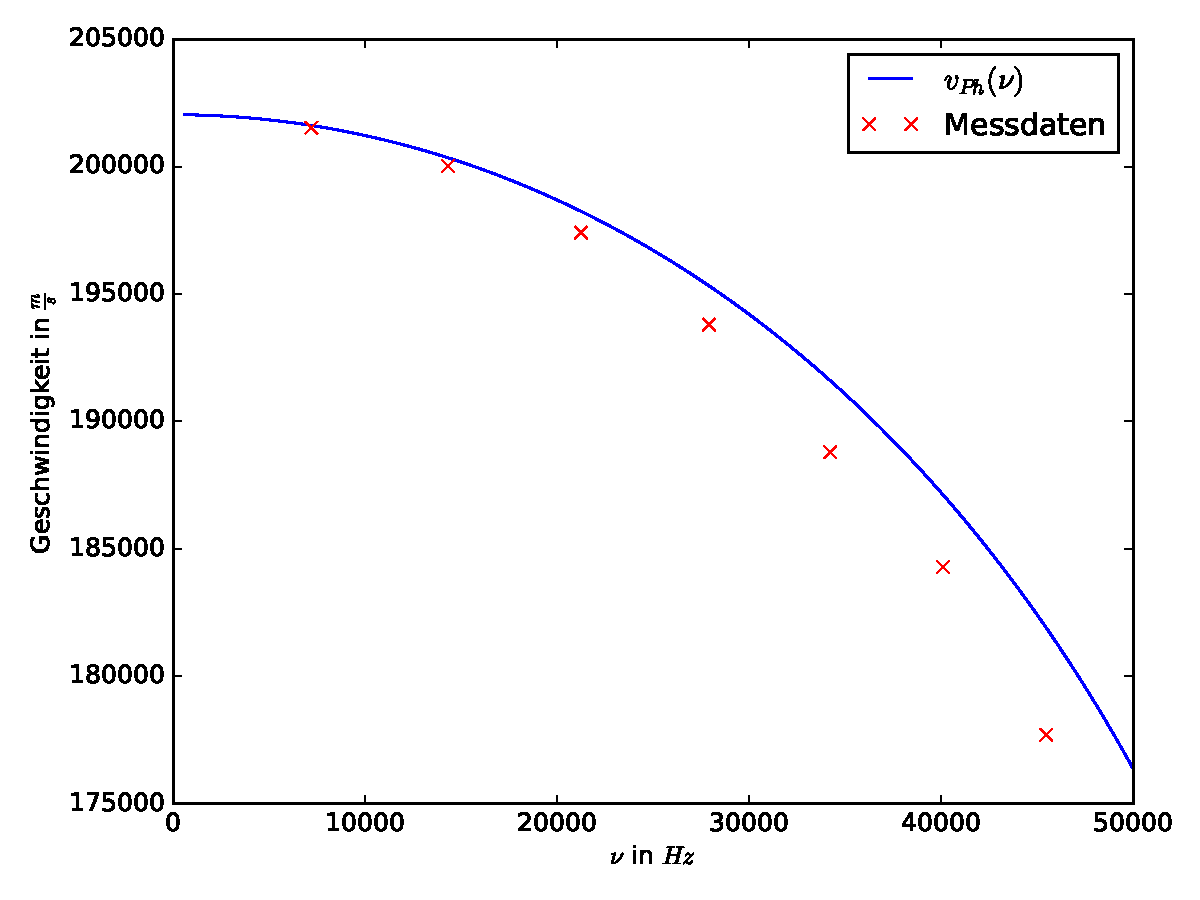
\includegraphics[width=\textwidth]{Phasengesch.pdf}
  \caption{Phasengeschwindigkeit}
  \label{fig:Phasengesch}
\end{figure}

In Abb. \ref{fig:Phasengesch} ist die Phasengeschwindigkeit gegenüber der
Frequenz aufgetragen. Die Theoriekurve wurde nach Formel \ref{eqn:RelationC}
berechnet. Es ist erkenntlich, dass die gemessenen Werte mit denen der
Theorie im Rahmen der Messunsicherheit übereinstimmen.
Die eingetragenen Messdaten sind aus Tabelle \ref{tab:Phasengesch} entnommen.

\subsection{Stehende Wellen}

Beim Messen der Spannungsamplituden der offenen $LC$-Kette ergeben sich die Diagramme
\ref{fig:Messungd1}, \ref{fig:Messungd2} und \ref{fig:Messunge}.

\begin{figure}
  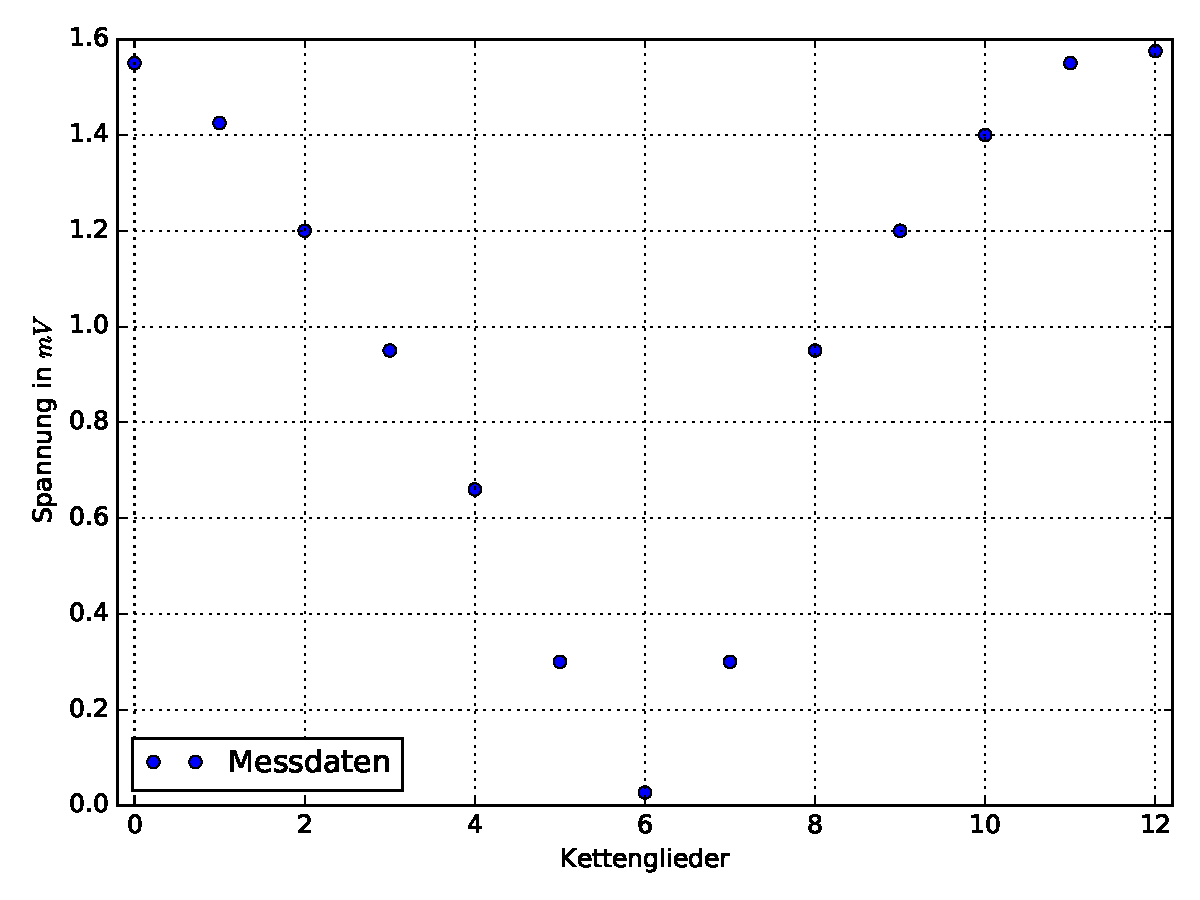
\includegraphics[width=\textwidth]{Messung_d_1.pdf}
  \caption{Erste Grundschwingung der offenen $LC$-Kettenschaltung bei $\nu = \SI{7133}{\hertz}$}
  \label{fig:Messungd1}
\end{figure}

Das Diagramm \ref{fig:Messungd1} zeigt die Messdaten der Spalte $\nu_C=\SI{7133}{\hertz}$
aus der Tabelle \ref{tab:stehendeWelle}. Die erste Grundschwigung ist deutlich
zu erkennen. Die Generatorfrequenz $\nu_C$ wurde auf die Frequenz
der ersten Eigenschwingung eingestellt, weshalb dieses Diagramm den Erwartungen
entspricht.

\FloatBarrier
\begin{figure}
  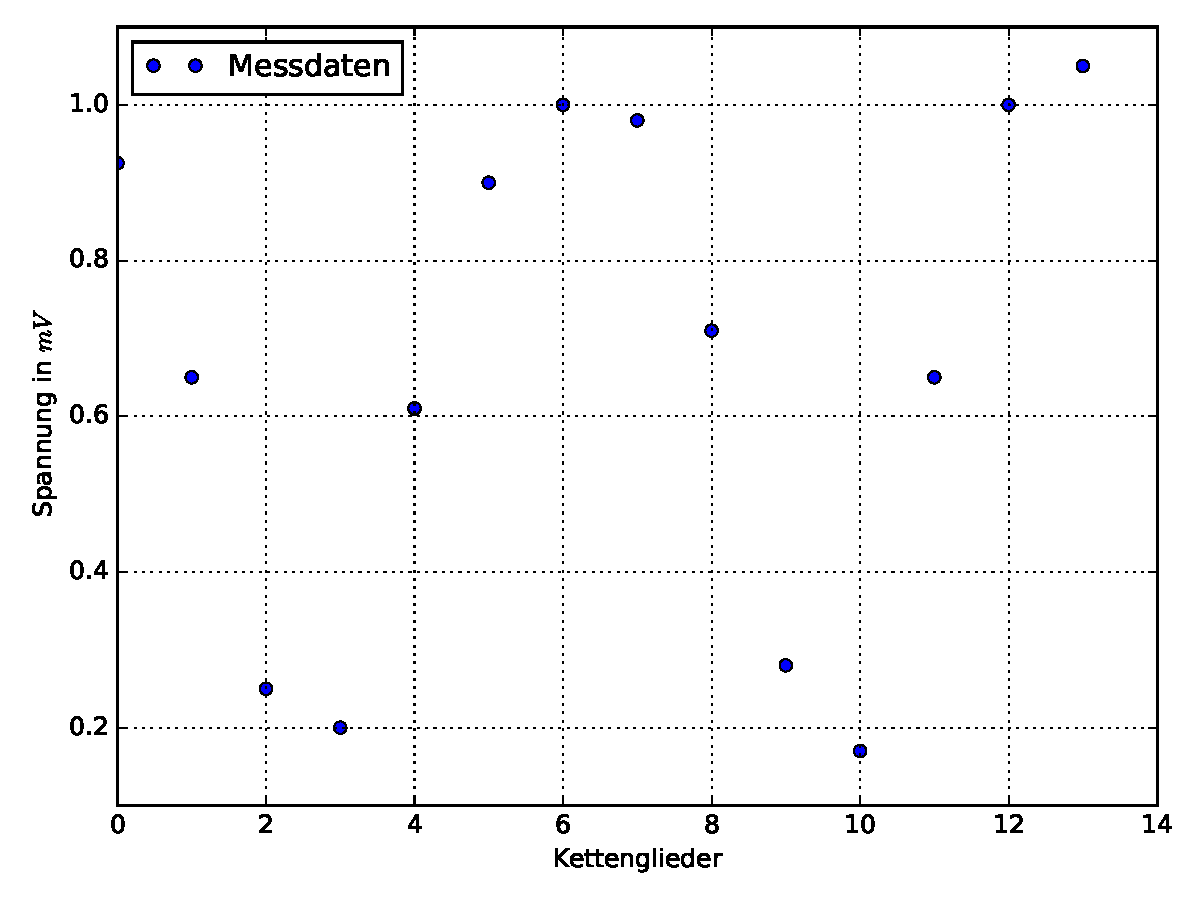
\includegraphics[width=\textwidth]{Messung_d_2.pdf}
  \caption{Zweite Grundschwingung der offenen $LC$-Kettenschaltung bei $\nu = \SI{14307}{\hertz}$}
  \label{fig:Messungd2}
\end{figure}

Die Darstellung der Werte aus Spalte $\nu_{C} = \SI{14307}{\hertz}$ von Tabelle \ref{tab:stehendeWelle}
ist in Diagramm \ref{fig:Messungd2} erfolgt. Die zweite Grundschwingung ist deutlich
erkennbar. Dies liegt daran, dass die Generatorfrequenz auf die zweite
Eigenfrequenz der Schaltung eingestellt wurde.

\FloatBarrier
\begin{figure}
  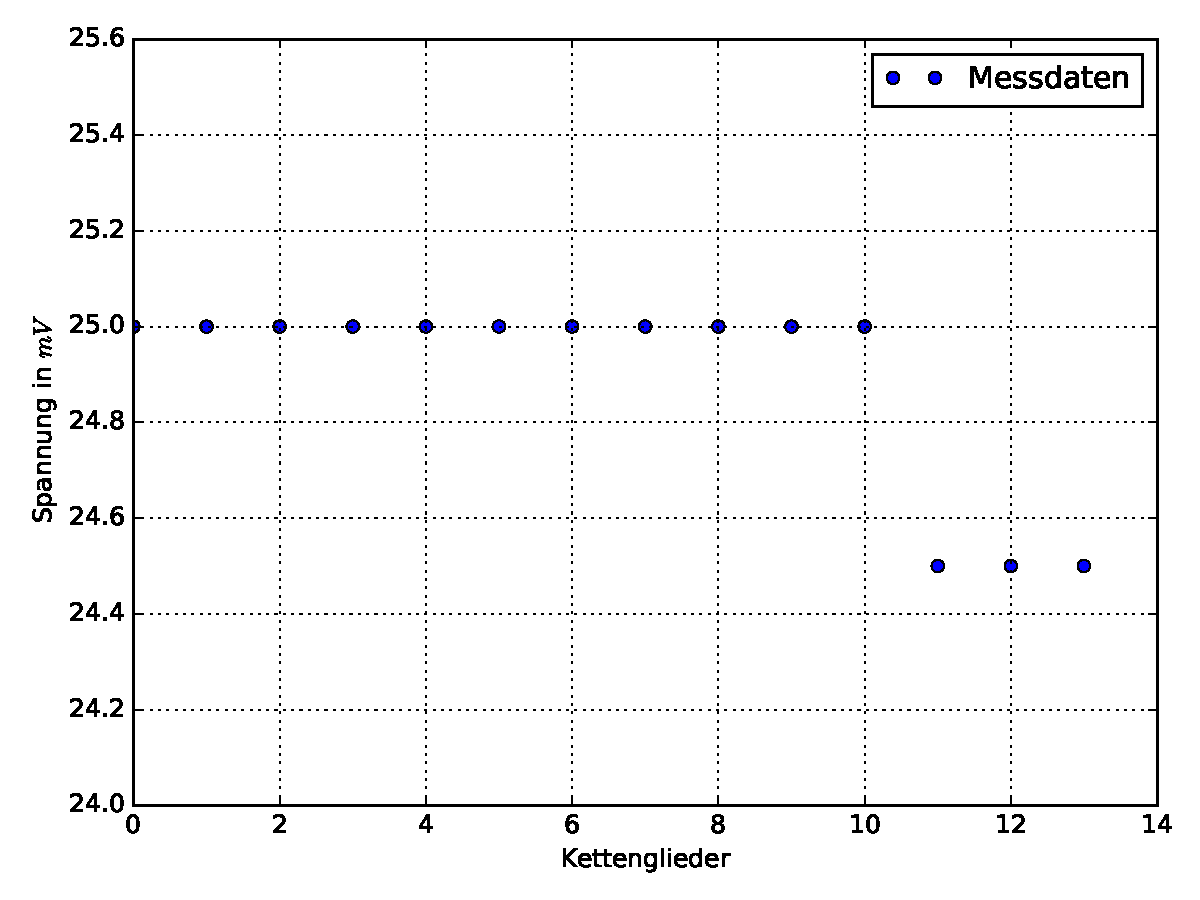
\includegraphics[width=\textwidth]{Messung_e.pdf}
  \caption{Abgeschlossene $LC-$Kettenschaltung bei $\nu = \SI{7337}{\hertz}$}
  \label{fig:Messunge}
\end{figure}

Das letzte Diagramm \ref{fig:Messunge} zeigt die Spannungsamplitunden
an den Kettengliedern bei der abgeschlossenen $LC$-Kette. Dafür wurden die
Daten der Tabelle \ref{tab:stehendeWelle} aus der Spalte von $\nu_{abge}$
bei einer Frequenz von $\SI{7337}{\hertz}$. Der Verlauf der Messdaten etspricht
den Erwartungen der Messung, da keine stehenden Welle erkenntlich sind.
Dies ergit sich auch aus den theoretischen Überlegungen über die
abgeschlossene Schaltung.

Die Messungen der Spannungsamplituden der offenen $LC$-Kettenschaltung, $LC_1C_2$-Kettenschaltung
und der abgeschlossenen $LC$-Kettenschaltung ergab die folgenden Werte. Die Angaben sind
in \si{\milli\volt}.

\FloatBarrier
\floatplacement{table}{htbp}
\begin{table}
 \centering
 \sisetup{table-format=1.3}
 \begin{tabular}[width=\textwidth]{S[table-format=1.0] S S S[table-format=2.0]}
     \toprule
      {Kettenglied} & {$\nu_C=\SI{7133}{\hertz}$} & {$\nu_{C} = \SI{14307}{\hertz}$} & {$\nu_{abge}=\SI{7337}{\hertz}$}\\
     \midrule
      1 & 1,55 & 0,925 & 25 \\
      2 & 1,425 & 0,65 & 25 \\
      3 & 1,2 & 0,25 & 25 \\
      4 & 0,95 & 0,2 & 25 \\
      5 & 0,66 & 0,61 & 25 \\
      6 & 0,3 & 0,9  & 25 \\
      7 & 0,027 & 1  & 25 \\
      8 & 0,3 & 0,98 & 25  \\
      9 & 0,95& 0,71  & 25 \\
      10 & 1,2 & 0,28 & 25 \\
      11 & 1,4 & 0,17 & 25 \\
      12 & 1,55 & 0,65 & 24,5 \\
      13 & 1,575 & 1 & 24,5 \\
    14 & \text{\,\,\,\,\,\,\,\,\,\,\,\,--} & 1,05 & 24,5 \\
      \bottomrule
\end{tabular}
  \caption{Messdaten der stehenden Welle}
  \label{tab:stehendeWelle}
\end{table}

\section{Diskussion}

Im Folgendem werden die Messergebnisse diskutiert.
Zunächst wird auf mögliche Fehlerquellen eingegangen, mit denen sich die Messungenauigkeiten
begründen lassen. Zum einen war das Einstellen des Wellenwiderstandes auf der
Eingangsseite (links) äußert unpräzise. Leichte Berührungen des Widerstandreglers
hatten schon enormen Einfluss auf den widergegebenen Widerstand.
Zudem konnten die gemessenen Frequenzen nur schwierig abgelesen werden, da der
Generator keine konstante Frequenz bereitgestellt hat. Die Frequenzen
können deshalb die Messergebnisse mit Fehlern behaftet haben.
Während des Zeichnens der Durchlasskurve durch den $XY$-Schreiber wurden Fixpunkte
an dem Diagramm gewählt, an denen die Frequenz zu bestimmen war. Die Abstandsmessung
der Fixpunkte wurde als fehlerfrei angenommen und das Messen der Frequenzen
erfolgte nicht parallel zum Zeichnen.
Insgesamt ist zu sagen, dass die verwendete Apparatur sehr alt ist und sehr
undurchsichtig wirkte.  Damit ist gemeint, dass nicht sichergestellt
war, ob alle angeschlossenen Bauteile funktionierten.
Die Induktivitäten und Kapazitäten der Apparatur wurden als fehlerfrei angenommen.\\
\\
Die Messergebnisse der Durchlasskurven sind in den Abbildungen \ref{fig:DispersionC}
und \ref{fig:DispersionC1C2} dargestellt. Es ist ersichtlich, dass
die Dispersionskurve der $LC$-Kette beinahe auf der Theoriekurve liegt.
Jedoch wird nicht die theoretische Grenzfrequenz in dem Aufbau erreicht.
Die Messung war nur bis zu einer relativen Phasenverschiebung pro Glied von
$\frac{\pi}{2}$ möglich. Die Lissajous-Figuren wurden bei allen höheren
Verschiebungen nicht mehr erkennbar. Die gemessene Dispersionskurve der
$LC_1C_2$-Kette ähnelt der Theoriekurve erkennbar, doch scheint sie um eine
Faktor verschoben zu sein. Es wird deutlich, dass der Anfang
der Kurve linear ist. Die Abweichungen der Messdaten von der Theoriekurve
sind durch die oben genannten Gründe erklärbar.\\ \\
Nun folgt eine Diskussion der Diagramme \ref{fig:Messungd1}, \ref{fig:Messungd2}
und \ref{fig:Messunge}. In den ersten Diagramm ist die 1. Eigenschwingung der
$LC$-Kettenschaltung zusehen. Die Gestalt der Eigenschwingung ist deutlich
zuerkennen. Abweichungen zu einer Theoriekurve der ersten Eigenschwingung
sind mit Frequenzschüben des Generators zu erklären.
Das zweite Diagramm zeigt die zweite Eigenschwingung des Systems, auch deren
Gestalt ist deutlich zu erkennen. Die beiden Knotenpunkte lassen sich erahnen.
Das an diesen Stellen keine wirklichen Knotenpunkte sitzen lässt sich wieder auf
Frequenzschübe des Generators zurückführen.
Das letzte Diagramm zeigt die abgeschlossenen $LC$-Kette bei einer Frequenz
von $\SI{7337}{\hertz}$. Es ist deutlich zuerkennen, dass sich keine sichtbare
Welle ausbreitet. Dies hängt damit zusammen, dass sich keine steheden Wellen
ausbilden. Die Abweichungen ab dem 11.
Kettenglied sind ebenfalls mit dem Wellenwiderstand zubegründen.

%\end{document}
